\documentclass[12pt]{article}
\usepackage{graphicx}
\usepackage{geometry}
\usepackage{setspace}
\usepackage{titlesec}
\usepackage{tocloft}
\usepackage{fancyhdr}
\usepackage{hyperref}
\usepackage{xcolor}
\usepackage[T1]{fontenc}
\usepackage[utf8]{inputenc}
\usepackage[ngerman]{babel}

\geometry{a4paper, margin=2.5cm}
\setstretch{1.5}
\titleformat{\section}[block]{\LARGE\bfseries\color{black}}{}{0em}{\filcenter}
\titlespacing*{\section}{0pt}{3.5ex plus 1ex minus .2ex}{2.3ex plus .2ex}
\renewcommand{\cftsecleader}{\cftdotfill{\cftdotsep}}
\renewcommand{\contentsname}{Inhaltsverzeichnis}
\renewcommand{\cftaftertoctitle}{\par\nobreak\bigskip\bigskip\bigskip}
\setlength{\cftbeforesecskip}{0.5em}
\setlength{\cftaftertoctitleskip}{2cm}
\hypersetup{
    colorlinks=true,
    linkcolor=blue,
    filecolor=magenta,
    urlcolor=cyan,
}

\pagestyle{fancy}
\fancyhf{}
\fancyhead[R]{\thepage}
\fancyhead[L]{\nouppercase{\leftmark}}
\renewcommand{\headrulewidth}{0pt}
\fancyfoot[C]{\thepage}
\renewcommand{\footrulewidth}{0pt}

\definecolor{lightgray}{RGB}{240,240,240}

\begin{document}

\begin{titlepage}
    \centering
    \vspace*{3cm}
    {\Huge\bfseries\textcolor{blue}{\MakeUppercase{ Liebe im Hörsaal }}\par}
    \vspace{0.5cm}
    {\Large\textit{ Maja Schmidt }\par}
    \vfill
    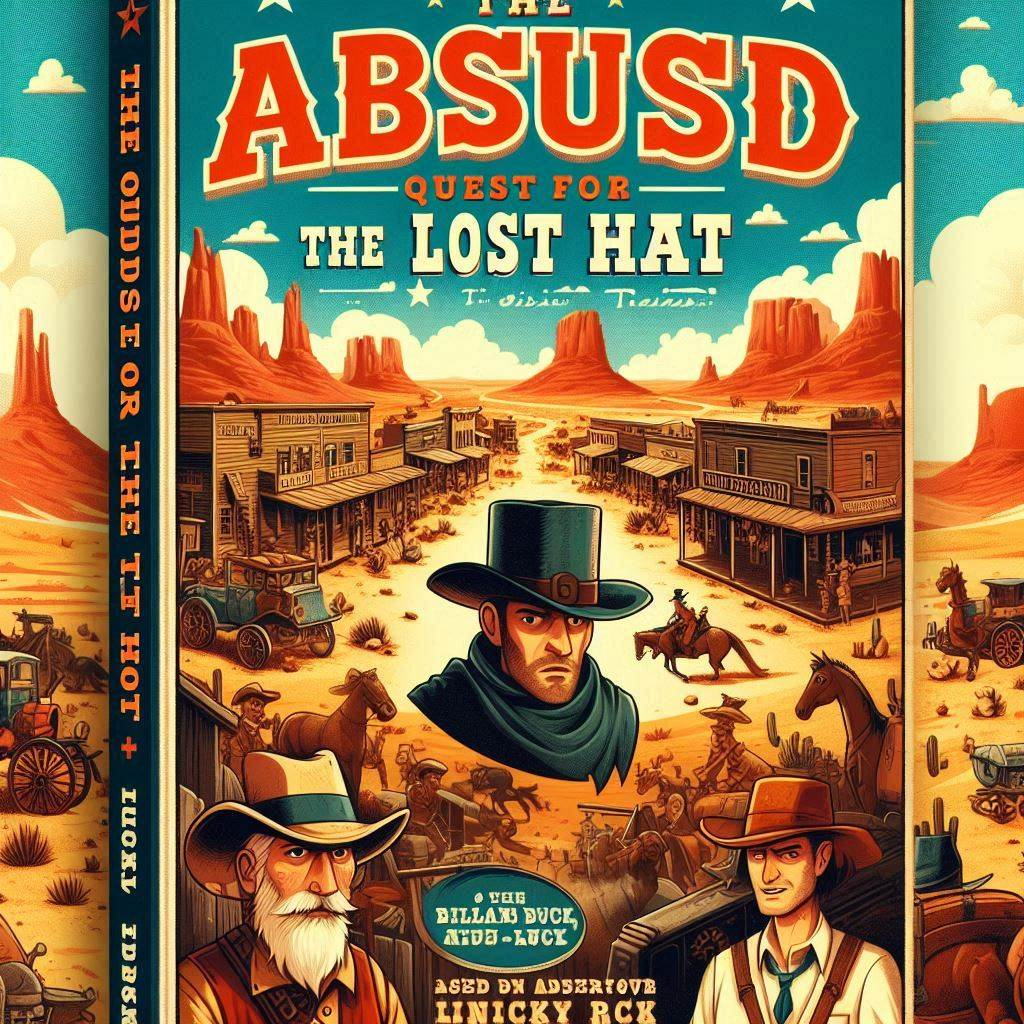
\includegraphics[width=0.9\textwidth]{ cover.jpg }
    \vfill
    \today
\end{titlepage}

\section*{Autorenvita}
\vspace{4cm}
Maja Schmidt ist eine bekannte und erfahrene Autorin von Liebesromanen, die sich auf das Thema Studentenleben spezialisiert hat. Mit ihrem humorvollen Schreibstil und ihrer Fähigkeit, lebendige und facettenreiche Charaktere zu erschaffen, hat sie sich eine treue Leserschaft aufgebaut. Ihre Geschichten sind geprägt von Romantik, Witz und authentischen Einblicken in das Leben junger Erwachsener.

\clearpage
\tableofcontents
\clearpage


\section{ Der erste Eindruck }
 Anna betrat den Hörsaal mit einem Stapel Bücher in der Hand und einem entschlossenen Blick. Sie war bereit für das neue Semester und wollte keinen Moment verschwenden. Als sie sich einen Platz in der ersten Reihe suchte, bemerkte sie einen jungen Mann, der lässig in der letzten Reihe saß und auf seinem Handy tippte. 

'Klassisch', dachte sie. 'Wieder so ein Typ, der das Studium nicht ernst nimmt.' 

Max, der junge Mann in der letzten Reihe, bemerkte Annas Blick und grinste. Er hatte schon viele wie sie gesehen – die Streber, die dachten, sie wüssten alles besser. 

'Hey, du da vorne!', rief er plötzlich. 'Kannst du mir sagen, ob das hier der Kurs für Literaturwissenschaften ist?' 

Anna drehte sich um und sah ihn mit hochgezogenen Augenbrauen an. 'Ja, das ist er. Und wenn du pünktlich wärst, wüsstest du das auch.' 

Max lachte. 'Entschuldigung, dass ich nicht so perfekt bin wie du.' 

Anna schnaubte und wandte sich wieder nach vorne. 'Unfassbar', murmelte sie. 

Der Professor betrat den Raum und begann mit der Vorlesung. Anna versuchte, sich zu konzentrieren, aber sie konnte das Gefühl nicht abschütteln, dass Max sie beobachtete. 

Nach der Vorlesung packte sie schnell ihre Sachen zusammen und wollte den Raum verlassen, als Max plötzlich neben ihr auftauchte. 

'Hey, ich bin Max', sagte er und streckte ihr die Hand entgegen. 

'Anna', antwortete sie kurz angebunden und ignorierte seine Hand. 

'Weißt du, Anna, du solltest dich nicht so stressen. Das Leben ist zu kurz, um es so ernst zu nehmen.' 

Anna funkelte ihn an. 'Und du solltest lernen, Verantwortung zu übernehmen. Das Leben ist kein Spiel.' 

Max zuckte mit den Schultern. 'Vielleicht hast du recht. Aber ein bisschen Spaß schadet auch nicht.' 

Anna schüttelte den Kopf und ging davon. 'Was für ein Idiot', dachte sie. 

Max sah ihr nach und grinste. 'Das wird interessant', murmelte er. Am nächsten Tag betrat Anna die Bibliothek, um an ihrem Essay zu arbeiten. Sie suchte sich einen ruhigen Platz in einer Ecke und breitete ihre Bücher aus. Gerade als sie sich in ihre Arbeit vertiefte, hörte sie eine vertraute Stimme. 

'Na, fleißig am Arbeiten?' 

Anna schaute auf und sah Max, der mit einem breiten Grinsen vor ihr stand. 

'Was machst du hier?', fragte sie genervt. 

'Ich dachte, ich könnte ein bisschen Gesellschaft gebrauchen', antwortete Max und setzte sich ungefragt neben sie. 

'Ich brauche keine Gesellschaft', erwiderte Anna scharf. 

Max zuckte mit den Schultern. 'Vielleicht nicht, aber ich schon. Außerdem, wer weiß, vielleicht kann ich dir ja helfen.' 

Anna schnaubte. 'Ich bezweifle, dass du mir bei Literaturwissenschaften helfen kannst.' 

Max grinste. 'Du wärst überrascht. Aber eigentlich wollte ich dich etwas fragen.' 

Anna seufzte. 'Was denn?' 

'Warum bist du immer so ernst? Ich meine, das Leben ist doch viel schöner, wenn man es ein bisschen lockerer nimmt.' 

Anna funkelte ihn an. 'Weil ich hart arbeiten muss, um meine Ziele zu erreichen. Nicht jeder hat das Glück, sich auf seinen Lorbeeren auszuruhen.' 

Max nickte langsam. 'Verstehe. Aber vielleicht solltest du trotzdem ab und zu mal durchatmen. Es könnte dir guttun.' 

Anna wollte gerade eine scharfe Antwort geben, als Lena, ihre Mitbewohnerin, auftauchte. 

'Hey Anna, ich habe dich überall gesucht!', sagte Lena und warf einen neugierigen Blick auf Max. 'Wer ist das?' 

'Oh, das ist Max. Er ist... ein Kommilitone', antwortete Anna zögernd. 

'Freut mich, dich kennenzulernen, Lena', sagte Max und reichte ihr die Hand. 

Lena lächelte. 'Freut mich auch. Anna, wir müssen los, wir haben noch einen Termin.' 

Anna packte schnell ihre Sachen zusammen und stand auf. 'Ja, richtig. Wir müssen gehen.' 

Max sah ihnen nach und rief: 'Bis bald, Anna!' 

Anna drehte sich nicht um, aber Lena konnte das leichte Lächeln auf ihrem Gesicht sehen. 'Interessanter Typ', bemerkte Lena. 

'Interessant ist nicht das Wort, das ich benutzen würde', murmelte Anna, aber sie konnte das Gefühl nicht abschütteln, dass Max vielleicht doch nicht so schlimm war, wie sie dachte. Am nächsten Tag im Hörsaal konnte Anna nicht anders, als Max' Anwesenheit zu bemerken. Er saß lässig in der hinteren Reihe, während sie sich wie immer in die vorderen Reihen setzte. Der Professor begann die Vorlesung, aber Annas Gedanken schweiften immer wieder zu Max ab. 

Nach der Vorlesung packte sie ihre Sachen zusammen, als Max plötzlich neben ihr auftauchte. 

'Hey Anna, hast du Lust, einen Kaffee trinken zu gehen?', fragte er mit einem charmanten Lächeln. 

Anna zögerte. 'Ich habe viel zu tun, Max.' 

'Komm schon, nur eine halbe Stunde. Du kannst doch nicht immer nur arbeiten.' 

Lena, die gerade vorbeikam, hörte das Gespräch und mischte sich ein. 'Anna, geh doch mit ihm. Ein bisschen Ablenkung tut dir gut.' 

Anna seufzte und gab schließlich nach. 'Na gut, aber nur eine halbe Stunde.' 

Im Café saßen sie sich gegenüber, und Max bestellte zwei Cappuccinos. 'Also, was machst du in deiner Freizeit, wenn du nicht gerade lernst?', fragte er neugierig. 

Anna zuckte mit den Schultern. 'Ich lese viel und gehe manchmal ins Theater. Und du?' 

'Ich spiele Gitarre und gehe gerne auf Partys. Aber ich kann auch mal ruhigere Abende genießen', antwortete Max. 

Anna konnte nicht anders, als zu lächeln. 'Das klingt... interessant.' 

Max grinste. 'Siehst du, wir haben doch mehr gemeinsam, als du denkst.' 

Plötzlich tauchte Tom auf und setzte sich ungefragt zu ihnen. 'Hey Max, was geht? Und wer ist die hübsche Dame?' 

Max stellte sie vor. 'Das ist Anna, eine Kommilitonin. Anna, das ist Tom, mein bester Freund.' 

Tom zwinkerte ihr zu. 'Freut mich, dich kennenzulernen, Anna.' 

Anna nickte höflich. 'Freut mich auch.' 

Die Unterhaltung verlief überraschend angenehm, und Anna merkte, dass sie sich in Max' Gesellschaft tatsächlich entspannen konnte. Als sie schließlich aufbrachen, fühlte sie sich leichter und weniger gestresst. 

'Bis bald, Anna', sagte Max, als sie sich verabschiedeten. 

Anna lächelte. 'Ja, bis bald.' 

Als sie nach Hause ging, konnte sie das Gefühl nicht abschütteln, dass Max vielleicht doch nicht so schlimm war, wie sie dachte.

\section{ Das gemeinsame Projekt }
 Am nächsten Morgen betrat Anna den Seminarraum und sah sofort Max, der lässig auf einem Stuhl saß und mit Tom plauderte. Sie setzte sich an ihren Platz und versuchte, die Nervosität zu unterdrücken, die sie seit dem gestrigen Kaffeeplausch verspürte. Der Professor trat ein und begann, die Projektgruppen zu verkünden.

'Anna Müller und Maximilian Becker', sagte er schließlich. Annas Herz sank. Sie war entsetzt, dass sie ausgerechnet mit Max zusammenarbeiten musste. Ein Blick zu Max zeigte ihr, dass er genauso wenig begeistert war.

'Na toll', murmelte Anna leise.

Max stand auf und kam zu ihr. 'Sieht so aus, als wären wir Partner', sagte er mit einem gezwungenen Lächeln.

Anna nickte widerwillig. 'Ja, sieht so aus.'

Lena, die neben Anna saß, versuchte, die Situation aufzuheitern. 'Das wird schon, Anna. Ihr werdet ein tolles Team sein.'

Tom grinste. 'Ja, und ich bin sicher, Max wird sich benehmen.'

Max verdrehte die Augen. 'Danke, Tom. Sehr hilfreich.'

Nach dem Seminar setzten sich Anna und Max zusammen, um das Projekt zu besprechen. Die ersten Minuten waren von unangenehmem Schweigen geprägt.

'Also, wie wollen wir das angehen?', fragte Anna schließlich.

Max zuckte mit den Schultern. 'Keine Ahnung. Vielleicht sollten wir erstmal die Aufgaben aufteilen.'

Anna nickte. 'Okay, ich kann die Recherche übernehmen und du kümmerst dich um die technische Umsetzung.'

Max stimmte zu. 'Klingt gut. Wann wollen wir uns das nächste Mal treffen?'

'Wie wäre es morgen in der Bibliothek?', schlug Anna vor.

'Passt. Bis dann', sagte Max und stand auf.

Als Anna nach Hause ging, konnte sie nicht anders, als sich Sorgen zu machen. Die Zusammenarbeit mit Max würde eine Herausforderung werden, aber sie war entschlossen, das Beste daraus zu machen. Am nächsten Tag trafen sich Anna und Max in der Bibliothek. Anna war wie immer pünktlich und hatte bereits einen Tisch mit allen notwendigen Materialien vorbereitet. Max kam fünf Minuten zu spät und trug ein verschmitztes Lächeln auf den Lippen.

'Guten Morgen', sagte er und setzte sich gegenüber von Anna.

'Guten Morgen', erwiderte Anna kühl. 'Lass uns anfangen. Ich habe einige Bücher über unser Thema gefunden.'

Max nickte und griff nach einem der Bücher. 'Klingt gut. Ich habe auch ein paar Ideen für die technische Umsetzung.'

Die ersten Minuten verliefen in angespannter Stille, unterbrochen nur vom Rascheln der Buchseiten und dem Tippen auf der Tastatur. Plötzlich stieß Max einen leisen Fluch aus.

'Was ist los?', fragte Anna und schaute auf.

'Ich habe gerade meinen Kaffee über meine Notizen verschüttet', sagte Max und hielt die durchnässten Blätter hoch.

Anna konnte sich ein Lächeln nicht verkneifen. 'Vielleicht solltest du weniger Kaffee trinken und mehr aufpassen.'

Max grinste. 'Vielleicht hast du recht. Aber ohne Kaffee funktioniere ich nicht.'

Lena und Tom, die zufällig in der Nähe waren, kamen vorbei und setzten sich zu ihnen. 'Wie läuft's bei euch?', fragte Lena.

'Fantastisch', sagte Max sarkastisch und zeigte auf seine nassen Notizen.

Tom lachte. 'Klassischer Max. Immer ein Chaos.'

Anna seufzte. 'Wir kommen schon irgendwie klar. Es ist nur... eine Herausforderung.'

Lena legte eine Hand auf Annas Schulter. 'Ihr schafft das. Ihr müsst nur einen Weg finden, miteinander auszukommen.'

Max nickte. 'Lena hat recht. Wir sollten versuchen, professionell zu bleiben.'

Anna stimmte zu. 'Okay, lass uns weitermachen. Wir haben viel zu tun.'

Die Gruppe arbeitete weiter, und obwohl es immer wieder zu kleinen Missgeschicken kam, begannen Anna und Max langsam, sich besser zu verstehen. Vielleicht, dachte Anna, war die Zusammenarbeit mit Max doch nicht so schlimm, wie sie befürchtet hatte. Die nächsten Tage verliefen ähnlich. Anna und Max trafen sich regelmäßig in der Bibliothek, und obwohl es immer wieder zu kleinen Missgeschicken kam, begannen sie, sich besser zu verstehen. Eines Abends, als sie wieder einmal bis spät in die Nacht arbeiteten, bemerkte Anna, dass Max ungewöhnlich still war.

'Alles in Ordnung?', fragte sie und schaute von ihrem Laptop auf.

Max seufzte. 'Ja, ich denke nur über das Projekt nach. Es ist schwieriger, als ich dachte.'

Anna nickte. 'Ja, es ist eine Herausforderung. Aber ich denke, wir machen Fortschritte.'

Max lächelte schwach. 'Du hast recht. Es ist nur... ich habe das Gefühl, dass ich dich manchmal enttäusche.'

Anna war überrascht. 'Warum denkst du das?'

'Weil du immer so organisiert und vorbereitet bist, und ich... na ja, ich bin das Gegenteil.'

Anna legte ihre Hand auf seine. 'Max, du hast viele gute Ideen und du bringst eine kreative Perspektive ein. Das ist genauso wichtig wie Organisation.'

Max schaute sie dankbar an. 'Danke, Anna. Das bedeutet mir viel.'

In diesem Moment kamen Lena und Tom wieder vorbei. 'Hey, ihr zwei! Immer noch am Arbeiten?', fragte Tom.

'Ja, wir versuchen, das Projekt voranzubringen', antwortete Anna.

Lena lächelte. 'Ihr macht das großartig. Und denkt daran, auch mal eine Pause zu machen.'

Max grinste. 'Gute Idee. Wie wäre es mit einem Kaffee?'

Anna lachte. 'Solange du ihn nicht wieder über deine Notizen kippst.'

Die Gruppe lachte und machte eine kurze Pause. Als sie zurückkamen, fühlten sich Anna und Max erfrischt und motiviert. Sie setzten ihre Arbeit fort und begannen, erste kleine Fortschritte zu machen. Vielleicht, dachte Anna, war die Zusammenarbeit mit Max doch nicht so schlimm, wie sie befürchtet hatte.

\section{ Die ersten Funken }
 Die nächsten Tage vergingen wie im Flug, und Anna und Max verbrachten immer mehr Zeit miteinander. Sie trafen sich nicht nur in der Bibliothek, sondern auch in Cafés und sogar im Park, um an ihrem Projekt zu arbeiten. Eines Nachmittags saßen sie in einem gemütlichen Café in der Altstadt von Heidelberg, als Max plötzlich aufblickte und sagte: 'Weißt du, Anna, ich habe nie gedacht, dass ich mich so gut mit jemandem verstehen könnte, der so anders ist als ich.'

Anna lächelte und nahm einen Schluck von ihrem Kaffee. 'Ja, ich hätte auch nie gedacht, dass wir so gut zusammenarbeiten können. Du bringst wirklich eine kreative Perspektive ein, die ich oft übersehe.'

Max grinste. 'Und du hältst mich organisiert, was definitiv nicht meine Stärke ist.'

In diesem Moment betraten Lena und Tom das Café und winkten ihnen zu. 'Hey, ihr zwei! Immer noch am Arbeiten?', rief Tom und setzte sich zu ihnen.

'Ja, aber wir machen Fortschritte', antwortete Anna und lächelte.

Lena nickte zustimmend. 'Das ist großartig zu hören. Ihr seid wirklich ein gutes Team.'

Max schaute Anna an und nickte. 'Ja, das sind wir.'

Nach einer Weile verabschiedeten sich Lena und Tom, um weiterzuziehen, und Anna und Max blieben allein zurück. Sie arbeiteten noch eine Weile weiter, bis Max plötzlich sagte: 'Weißt du, Anna, ich habe das Gefühl, dass wir nicht nur an diesem Projekt arbeiten, sondern auch an etwas anderem.'

Anna schaute ihn fragend an. 'Was meinst du?'

Max zögerte einen Moment, bevor er antwortete: 'Ich meine, dass wir uns besser kennenlernen und vielleicht sogar Freunde werden.'

Anna lächelte. 'Ja, das denke ich auch. Und wer weiß, vielleicht sogar mehr als das.'

Max grinste breit. 'Vielleicht.'

In diesem Moment fühlte Anna, wie sich etwas zwischen ihnen veränderte. Es war, als ob ein unsichtbares Band sie näher zusammenbrachte. Sie wusste, dass dies der Anfang von etwas Besonderem war. Ein paar Tage später trafen sich Anna und Max in der Bibliothek, um weiter an ihrem Projekt zu arbeiten. Die Atmosphäre war ruhig, und das Licht der Nachmittagssonne fiel durch die hohen Fenster. Sie saßen an einem Tisch, umgeben von hohen Bücherregalen, und arbeiteten konzentriert.

Plötzlich stieß Max einen leisen Seufzer aus. 'Ich glaube, ich brauche eine Pause. Mein Kopf raucht schon.'

Anna lächelte und nickte. 'Ja, eine kleine Pause klingt gut. Wollen wir einen Spaziergang machen?'

Max' Augen leuchteten auf. 'Das ist eine großartige Idee. Lass uns zum Philosophenweg gehen. Die Aussicht dort ist fantastisch.'

Sie packten ihre Sachen zusammen und machten sich auf den Weg. Der Philosophenweg war ein malerischer Pfad, der sich entlang des Neckars erstreckte und einen atemberaubenden Blick auf die Altstadt und das Schloss bot. Während sie gingen, unterhielten sie sich über alles Mögliche – von ihren Studienfächern bis hin zu ihren Lieblingsfilmen.

'Weißt du, ich habe nie gedacht, dass Informatik so interessant sein könnte', sagte Anna und schaute Max an. 'Du hast wirklich eine Leidenschaft dafür.'

Max lächelte. 'Ja, ich liebe es, Probleme zu lösen und neue Dinge zu erschaffen. Aber ich muss zugeben, dass Literaturwissenschaften auch faszinierend sind. Du hast mir eine ganz neue Welt eröffnet.'

Anna lachte. 'Das freut mich zu hören. Vielleicht sollten wir öfter über unsere Interessen sprechen. Es gibt so viel, was wir voneinander lernen können.'

Max nickte zustimmend. 'Absolut. Und wer weiß, vielleicht können wir unsere Fähigkeiten sogar kombinieren und etwas Großartiges schaffen.'

Sie erreichten eine Bank mit Blick auf den Fluss und setzten sich. Die Stille war angenehm, und sie genossen den Moment. Nach einer Weile sagte Max leise: 'Anna, ich bin wirklich froh, dass wir dieses Projekt zusammen machen. Es hat mir gezeigt, dass man manchmal die besten Dinge findet, wenn man es am wenigsten erwartet.'

Anna lächelte und legte ihre Hand auf seine. 'Ich bin auch froh, Max. Ich denke, wir sind auf dem besten Weg, nicht nur ein großartiges Projekt, sondern auch eine großartige Freundschaft zu entwickeln.'

Max schaute ihr in die Augen und nickte. 'Ja, das denke ich auch.' Als sie zurück zur Bibliothek gingen, fühlte sich die Atmosphäre zwischen Anna und Max verändert an. Es war, als ob der Spaziergang eine unsichtbare Barriere zwischen ihnen abgebaut hatte. Sie setzten sich wieder an ihren Tisch und begannen, weiter an ihrem Projekt zu arbeiten.

Nach einer Weile kam Lena vorbei, um nach Anna zu sehen. 'Hey Anna, wie läuft's mit dem Projekt?'

Anna lächelte. 'Es läuft gut, Lena. Max und ich machen Fortschritte.'

Lena warf Max einen prüfenden Blick zu und grinste. 'Das freut mich zu hören. Ich wollte nur kurz Hallo sagen. Ich muss zurück zu meiner eigenen Arbeit. Viel Erfolg euch beiden!'

Nachdem Lena gegangen war, sah Max Anna an. 'Lena scheint eine tolle Freundin zu sein.'

Anna nickte. 'Ja, das ist sie. Sie ist immer für mich da.'

Tom tauchte plötzlich auf und setzte sich neben Max. 'Hey, was geht ab? Ich dachte, ich schau mal vorbei und sehe, wie ihr vorankommt.'

Max lachte. 'Wir kommen gut voran, Tom. Danke, dass du fragst.'

Tom grinste und zwinkerte Anna zu. 'Pass gut auf Max auf, Anna. Er kann manchmal ein bisschen chaotisch sein.'

Anna lachte. 'Keine Sorge, Tom. Ich habe alles im Griff.'

Tom verabschiedete sich und ließ die beiden wieder allein. Anna und Max arbeiteten weiter, und die Zeit verging wie im Flug. Als sie schließlich ihre Sachen zusammenpackten, um zu gehen, sagte Max: 'Weißt du, Anna, ich habe das Gefühl, dass wir ein wirklich gutes Team sind.'

Anna lächelte. 'Ja, das denke ich auch. Ich freue mich auf die nächsten Schritte unseres Projekts.'

Max nickte. 'Ich auch. Und wer weiß, vielleicht wird aus diesem Projekt noch etwas viel Größeres.'

Anna sah ihn an und spürte, wie sich ein warmes Gefühl in ihr ausbreitete. 'Ja, vielleicht.'

\section{ Der große Streit }
 Anna und Max saßen in der Bibliothek, vertieft in ihre Arbeit. Die Atmosphäre war angespannt, als ob eine unsichtbare Wolke über ihnen hing. Anna warf einen Blick auf Max, der konzentriert auf seinen Laptop starrte. Sie seufzte leise und versuchte, sich wieder auf ihre Notizen zu konzentrieren.

Plötzlich brach Max die Stille. 'Anna, ich denke, wir sollten diesen Teil des Projekts anders angehen. Dein Ansatz ist zu theoretisch.'

Anna hob den Kopf und sah ihn an. 'Was meinst du damit? Mein Ansatz ist fundiert und basiert auf soliden Quellen.'

Max schüttelte den Kopf. 'Ja, aber er ist nicht praktisch genug. Wir müssen etwas Innovatives präsentieren, nicht nur Theorie.'

Anna spürte, wie sich Ärger in ihr aufbaute. 'Du verstehst einfach nicht, wie wichtig die theoretische Grundlage ist. Ohne sie ist unser Projekt nichts wert.'

Max' Augen blitzten auf. 'Und du verstehst nicht, dass wir etwas Greifbares liefern müssen. Etwas, das die Leute beeindruckt.'

Die Spannung zwischen ihnen wuchs, und bevor sie es wussten, waren sie in einen hitzigen Streit verwickelt. Ihre Stimmen wurden lauter, und einige Studenten in der Nähe warfen ihnen genervte Blicke zu.

Lena, die gerade vorbeikam, blieb stehen und sah die beiden besorgt an. 'Hey, was ist hier los?'

Anna drehte sich zu ihr um, ihre Augen funkelten vor Wut. 'Max denkt, dass meine Arbeit nicht gut genug ist.'

Max hob die Hände in einer beschwichtigenden Geste. 'Das habe ich nicht gesagt. Ich denke nur, dass wir einen anderen Ansatz brauchen.'

Tom, der ebenfalls in der Nähe war, kam hinzu und legte eine Hand auf Max' Schulter. 'Beruhigt euch, Leute. Streiten bringt uns nicht weiter.'

Anna stand abrupt auf. 'Ich brauche eine Pause. Ich kann so nicht arbeiten.' Sie schnappte sich ihre Sachen und verließ die Bibliothek, ohne zurückzublicken.

Max sah ihr nach und seufzte tief. 'Das lief nicht gut.'

Lena legte eine Hand auf seine Schulter. 'Gib ihr etwas Zeit. Sie wird sich beruhigen.'

Tom nickte zustimmend. 'Ja, und dann könnt ihr in Ruhe darüber reden. Ihr seid ein gutes Team, ihr schafft das.'

Max nickte langsam, aber die Zweifel nagten an ihm. War ihre Zusammenarbeit wirklich so gut, wie er dachte? Max blieb noch eine Weile in der Bibliothek sitzen, doch seine Gedanken kreisten um den Streit mit Anna. Schließlich packte er seine Sachen zusammen und machte sich auf den Weg zum Studentenwohnheim. Er hoffte, dass er Anna dort antreffen würde, um die Sache zu klären.

Als er das Wohnheim erreichte, sah er Lena und Tom im Gemeinschaftsraum sitzen. Lena winkte ihn heran. 'Hey Max, wie geht's dir?'

Max seufzte. 'Nicht so gut. Ich mache mir Sorgen um Anna. Ich glaube, ich habe es wirklich vermasselt.'

Tom klopfte ihm auf die Schulter. 'Mach dir nicht zu viele Gedanken. Anna ist stark, sie wird sich beruhigen. Vielleicht solltest du ihr einfach etwas Zeit geben.'

Lena nickte zustimmend. 'Ja, und wenn du bereit bist, könnt ihr in Ruhe darüber reden. Ihr müsst nur einen Weg finden, eure unterschiedlichen Ansätze zu kombinieren.'

Max setzte sich zu ihnen. 'Ich weiß, aber ich habe das Gefühl, dass wir uns immer wieder in die Haare kriegen. Vielleicht sind wir einfach zu unterschiedlich.'

Lena lächelte aufmunternd. 'Unterschiede können auch eine Stärke sein, Max. Ihr müsst nur lernen, sie zu nutzen.'

In diesem Moment öffnete sich die Tür, und Anna trat ein. Sie sah überrascht aus, als sie Max dort sitzen sah, aber sie setzte sich zu ihnen. 'Ich denke, wir müssen reden.'

Max nickte. 'Ja, das müssen wir. Es tut mir leid, dass ich so auf deinen Ansatz reagiert habe. Ich wollte deine Arbeit nicht abwerten.'

Anna seufzte. 'Ich weiß, und es tut mir leid, dass ich so wütend geworden bin. Vielleicht sollten wir wirklich versuchen, unsere Ansätze zu kombinieren.'

Tom grinste. 'Das klingt nach einem Plan. Ihr seid beide klug und talentiert. Zusammen könnt ihr etwas Großartiges schaffen.'

Lena fügte hinzu: 'Und wir sind hier, um euch zu unterstützen. Ihr seid nicht allein.'

Anna und Max sahen sich an und lächelten. 'Okay, lass es uns versuchen', sagte Anna. 'Aber wir müssen wirklich zusammenarbeiten und aufeinander hören.'

Max nickte. 'Abgemacht. Wir schaffen das.' Anna und Max saßen sich gegenüber, die Spannung zwischen ihnen war greifbar. Lena und Tom hatten sich diskret zurückgezogen, um ihnen Raum zu geben.

'Also, wie wollen wir das angehen?' fragte Anna und brach das Schweigen.

Max lehnte sich zurück und dachte nach. 'Vielleicht sollten wir uns auf unsere Stärken konzentrieren. Du bist gut im Strukturieren und Planen, und ich kann die technischen Aspekte übernehmen.'

Anna nickte langsam. 'Das klingt vernünftig. Aber wir müssen auch lernen, besser zu kommunizieren. Ich habe das Gefühl, dass wir oft aneinander vorbeireden.'

Max seufzte. 'Ja, das stimmt. Vielleicht sollten wir regelmäßige Check-ins einplanen, um sicherzustellen, dass wir auf dem gleichen Stand sind.'

Anna lächelte leicht. 'Das ist eine gute Idee. Und wir sollten uns auch die Zeit nehmen, die Arbeit des anderen zu schätzen. Ich weiß, dass du viel Mühe in das Projekt steckst, auch wenn ich es nicht immer zeige.'

Max erwiderte ihr Lächeln. 'Danke, Anna. Das bedeutet mir viel. Und ich werde versuchen, deine Perspektive mehr zu berücksichtigen.'

In diesem Moment kamen Lena und Tom zurück. 'Na, habt ihr eine Lösung gefunden?' fragte Tom neugierig.

Anna nickte. 'Ja, wir haben einen Plan. Wir werden unsere Stärken nutzen und besser kommunizieren.'

Lena strahlte. 'Das klingt großartig! Ihr werdet das schaffen, da bin ich sicher.'

Tom klopfte Max auf den Rücken. 'Siehst du, ich habe dir doch gesagt, dass ihr das hinkriegt.'

Max lachte. 'Ja, du hattest recht. Danke, dass ihr für uns da seid.'

Anna sah in die Runde und fühlte sich zum ersten Mal seit langem erleichtert. 'Danke, Leute. Wir werden das gemeinsam durchstehen.'

Mit neuem Mut und einem klaren Plan machten sich Anna und Max daran, ihre Zusammenarbeit zu verbessern und das Projekt erfolgreich abzuschließen.

\section{ Die Versöhnung }
 Anna und Max saßen sich in einem kleinen Café gegenüber. Die Atmosphäre war angespannt, aber beide wussten, dass dieses Gespräch notwendig war.

'Ich möchte mich entschuldigen, Max,' begann Anna und schaute ihn direkt an. 'Ich war unfair und habe dich nicht wirklich zu Wort kommen lassen.'

Max nickte langsam. 'Ich habe auch Fehler gemacht. Ich hätte mehr auf dich hören sollen und nicht einfach mein Ding durchziehen.'

Anna seufzte erleichtert. 'Es ist gut, dass wir das klären. Wir müssen einen Weg finden, besser zusammenzuarbeiten.'

'Ja, das müssen wir,' stimmte Max zu. 'Vielleicht sollten wir uns regelmäßige Zeiten zum Reden einplanen, damit wir Missverständnisse vermeiden.'

'Gute Idee,' sagte Anna und lächelte leicht. 'Und wir sollten uns auch gegenseitig mehr unterstützen. Ich weiß, dass du viel Mühe in das Projekt steckst.'

Max erwiderte ihr Lächeln. 'Danke, Anna. Das bedeutet mir viel. Und ich werde versuchen, deine Perspektive mehr zu berücksichtigen.'

In diesem Moment betraten Lena und Tom das Café. 'Na, habt ihr eine Lösung gefunden?' fragte Tom neugierig.

Anna nickte. 'Ja, wir haben einen Plan. Wir werden unsere Stärken nutzen und besser kommunizieren.'

Lena strahlte. 'Das klingt großartig! Ihr werdet das schaffen, da bin ich sicher.'

Tom klopfte Max auf den Rücken. 'Siehst du, ich habe dir doch gesagt, dass ihr das hinkriegt.'

Max lachte. 'Ja, du hattest recht. Danke, dass ihr für uns da seid.'

Anna sah in die Runde und fühlte sich zum ersten Mal seit langem erleichtert. 'Danke, Leute. Wir werden das gemeinsam durchstehen.'

Mit neuem Mut und einem klaren Plan machten sich Anna und Max daran, ihre Zusammenarbeit zu verbessern und das Projekt erfolgreich abzuschließen. Anna und Max saßen wieder in der Bibliothek, diesmal mit einem klaren Plan und einer neuen Einstellung. Sie hatten beschlossen, ihre Stärken zu nutzen und sich gegenseitig zu unterstützen.

'Also, wie wollen wir das angehen?' fragte Max und schaute Anna erwartungsvoll an.

'Ich denke, wir sollten zuerst die Aufgaben aufteilen, basierend auf unseren Stärken,' schlug Anna vor. 'Du bist großartig in der technischen Umsetzung, und ich kann mich um die Recherche und das Schreiben kümmern.'

Max nickte zustimmend. 'Klingt gut. Und wir sollten regelmäßige Check-ins einplanen, um sicherzustellen, dass wir auf dem richtigen Weg sind.'

'Genau,' stimmte Anna zu. 'Vielleicht jeden zweiten Tag?'

'Perfekt,' sagte Max und lächelte. 'Ich bin froh, dass wir das klären konnten.'

In diesem Moment kamen Lena und Tom mit zwei großen Tassen Kaffee auf sie zu. 'Hier, eine kleine Stärkung für die fleißigen Arbeiter,' sagte Lena und stellte die Tassen vor ihnen ab.

'Danke, Lena,' sagte Anna und nahm einen Schluck. 'Das ist genau das, was wir jetzt brauchen.'

Tom setzte sich neben Max und grinste. 'Also, was ist der Plan?'

'Wir haben beschlossen, unsere Aufgaben aufzuteilen und regelmäßige Check-ins zu machen,' erklärte Max. 'Und wir werden uns gegenseitig mehr unterstützen.'

'Klingt nach einem soliden Plan,' sagte Tom und klopfte Max auf die Schulter. 'Ihr werdet das rocken.'

Lena nickte zustimmend. 'Und wenn ihr Hilfe braucht, sind wir da.'

Anna lächelte dankbar. 'Danke, Leute. Das bedeutet uns viel.'

Mit neuem Elan und einem klaren Plan machten sich Anna und Max an die Arbeit. Sie fühlten sich motiviert und bereit, die Herausforderungen gemeinsam zu meistern. Die Atmosphäre war jetzt viel entspannter, und sie konnten sich besser auf ihre Aufgaben konzentrieren. Es war der Beginn einer neuen Phase ihrer Zusammenarbeit und ihrer Beziehung. Während Anna und Max konzentriert arbeiteten, entstand eine neue Dynamik zwischen ihnen. Sie lachten über kleine Missgeschicke und halfen sich gegenseitig, wenn einer von ihnen feststeckte. Die Atmosphäre war entspannt und produktiv.

'Weißt du, Max,' sagte Anna plötzlich und legte ihren Stift beiseite, 'ich hätte nie gedacht, dass wir so gut zusammenarbeiten könnten.'

Max sah sie an und lächelte. 'Ich auch nicht. Aber ich bin froh, dass wir es geschafft haben, unsere Differenzen beiseite zu legen.'

Lena, die in der Nähe saß und ihre eigenen Studienunterlagen durchging, konnte sich ein Grinsen nicht verkneifen. 'Ihr zwei seid wirklich ein gutes Team. Vielleicht solltet ihr öfter zusammenarbeiten.'

Tom, der gerade von einer kurzen Pause zurückkam, setzte sich wieder zu ihnen. 'Ja, und wer weiß, vielleicht wird aus euch beiden ja noch mehr als nur ein gutes Team.'

Anna und Max tauschten einen kurzen, verlegenen Blick, bevor sie beide in Gelächter ausbrachen. 'Lass uns erst mal das Projekt abschließen, Tom,' sagte Max und schüttelte den Kopf.

'Genau,' stimmte Anna zu. 'Aber danke für die Unterstützung, ihr beiden. Es bedeutet uns wirklich viel.'

Lena nickte. 'Kein Problem. Wir sind immer für euch da.'

Mit neuer Energie und einem klaren Ziel vor Augen setzten Anna und Max ihre Arbeit fort. Sie fühlten sich nicht nur als Team, sondern auch als Freunde, die sich gegenseitig unterstützten und aufeinander verlassen konnten. Es war der Beginn einer neuen Phase ihrer Zusammenarbeit und ihrer Beziehung, und beide waren gespannt, wohin diese Reise sie führen würde.

\section{ Die Party }
 Anna und Max saßen in der Bibliothek und arbeiteten konzentriert an ihrem Projekt, als Lena plötzlich hereinstürmte. 'Hey, ihr zwei! Habt ihr schon von der großen Party heute Abend gehört? Die ganze Uni spricht darüber!'

Max hob den Kopf und grinste. 'Eine Party? Klingt nach einer guten Gelegenheit, mal den Kopf freizubekommen.'

Anna runzelte die Stirn. 'Ich weiß nicht, ob das eine gute Idee ist. Wir haben noch so viel zu tun.'

Tom, der gerade hereinkam, klopfte Anna auf die Schulter. 'Komm schon, Anna. Ein bisschen Spaß hat noch niemandem geschadet. Außerdem, wer weiß, vielleicht wird es ja ganz lustig.'

Lena nickte eifrig. 'Ja, und es wäre eine gute Gelegenheit, mal abzuschalten und die anderen Studenten besser kennenzulernen.'

Anna seufzte und sah zu Max, der sie mit einem hoffnungsvollen Blick ansah. 'Na gut, aber nur für ein paar Stunden. Wir müssen morgen früh wieder fit sein.'

'Abgemacht!' rief Max und Lena gleichzeitig und lachten.

Später am Abend trafen sich die vier vor dem Studentenwohnheim. Lena trug ein schickes Kleid, während Tom in einem lässigen Hemd und Jeans erschien. Anna und Max hatten sich ebenfalls in Schale geworfen, und Anna konnte nicht anders, als Max' charmantes Lächeln zu bemerken.

'Bereit für eine unvergessliche Nacht?' fragte Tom und führte die Gruppe zur Party.

Die Party war in vollem Gange, als sie ankamen. Musik dröhnte aus den Lautsprechern, und die Tanzfläche war voller Studenten, die ausgelassen feierten. Anna fühlte sich zunächst etwas unwohl, aber Max nahm ihre Hand und zog sie auf die Tanzfläche. 'Komm schon, Anna. Lass uns ein bisschen Spaß haben.'

Anna lachte und ließ sich von der Musik mitreißen. Sie tanzten und lachten, und für einen Moment vergaß sie all ihre Sorgen und den Stress des Projekts. Lena und Tom gesellten sich zu ihnen, und die vier Freunde genossen die ausgelassene Stimmung.

Es war eine Nacht, die sie so schnell nicht vergessen würden. Die Stunden vergingen wie im Flug, und die Party wurde immer ausgelassener. Anna und Max hatten sich in eine Ecke zurückgezogen, um sich ein wenig auszuruhen. 'Ich hätte nie gedacht, dass ich so viel Spaß haben würde', sagte Anna und lächelte Max an.

'Ich auch nicht', erwiderte Max und nahm einen Schluck von seinem Getränk. 'Aber ich bin froh, dass du mitgekommen bist.'

In diesem Moment kam Lena mit zwei Gläsern in der Hand auf sie zu. 'Hier, das müsst ihr probieren! Es ist der beste Cocktail des Abends.'

Anna nahm ein Glas und nippte daran. 'Wow, das ist wirklich gut!'

Tom gesellte sich zu ihnen und legte einen Arm um Lena. 'Ich habe gerade mit ein paar Leuten gesprochen, die uns zu einem Trinkspiel einladen wollen. Seid ihr dabei?'

Max grinste. 'Klar, warum nicht?'

Anna zögerte kurz, aber als sie die erwartungsvollen Blicke ihrer Freunde sah, nickte sie. 'Okay, aber nur ein Spiel.'

Das Trinkspiel entpuppte sich als eine lustige Runde 'Wahrheit oder Pflicht'. Die Gruppe lachte und scherzte, während sie sich gegenseitig herausforderten. Als Anna an der Reihe war, wählte sie 'Wahrheit'.

'Okay, Anna', sagte Tom mit einem schelmischen Grinsen. 'Was war dein erster Eindruck von Max?'

Anna errötete leicht und warf Max einen kurzen Blick zu. 'Um ehrlich zu sein, dachte ich, er wäre ein arroganter Schnösel.'

Die Gruppe brach in Gelächter aus, und Max tat so, als wäre er tief verletzt. 'Autsch, das hat gesessen!'

Anna lachte und legte eine Hand auf seine Schulter. 'Aber ich habe schnell gemerkt, dass ich mich geirrt habe.'

Max lächelte sie an, und für einen Moment schien die Welt um sie herum stillzustehen. Lena und Tom tauschten einen wissenden Blick aus und beschlossen, den beiden etwas Raum zu geben.

'Kommt, lasst uns noch ein bisschen tanzen', schlug Lena vor und zog Tom mit sich auf die Tanzfläche.

Anna und Max blieben zurück und genossen die ruhige Atmosphäre. 'Ich bin froh, dass wir heute Abend hier sind', sagte Max leise.

'Ich auch', antwortete Anna und lehnte sich an seine Schulter. 'Ich auch.' Anna und Max saßen noch immer in ihrer Ecke, als die Musik plötzlich langsamer wurde und ein romantisches Lied zu spielen begann. Max sah Anna an und fragte: 'Möchtest du tanzen?'

Anna zögerte kurz, dann nickte sie. 'Ja, gerne.'

Sie standen auf und gingen zur Tanzfläche, wo sie sich in die Arme nahmen und langsam im Takt der Musik wiegten. Max hielt Anna sanft, und sie legte ihren Kopf auf seine Schulter. Für einen Moment schien die Welt um sie herum zu verschwinden.

'Weißt du, ich hätte nie gedacht, dass wir uns so gut verstehen würden', sagte Max leise.

Anna lächelte. 'Ich auch nicht. Aber ich bin froh, dass wir es tun.'

In diesem Moment kam Lena wieder auf sie zu, diesmal ohne Tom. 'Hey, ihr zwei, alles in Ordnung?'

Max nickte. 'Ja, alles bestens. Wo ist Tom?'

Lena grinste. 'Er ist gerade auf der Tanzfläche und zeigt seine besten Moves. Ihr solltet ihn sehen!'

Anna lachte. 'Das klingt nach Tom.'

Lena zwinkerte ihnen zu. 'Ich lasse euch dann mal wieder allein. Genießt den Abend!' Sie drehte sich um und verschwand in der Menge.

Max und Anna tanzten weiter, verloren in ihrem eigenen kleinen Universum. Schließlich endete das Lied, und sie blieben noch einen Moment stehen, bevor sie sich langsam voneinander lösten.

'Danke für den Tanz', sagte Anna leise.

'Danke, dass du mit mir getanzt hast', erwiderte Max und lächelte sie an.

Sie gingen zurück zu ihrer Ecke und setzten sich wieder. Die Party ging weiter, aber für Anna und Max war dieser Moment etwas Besonderes. Sie wussten, dass sich etwas zwischen ihnen verändert hatte, und sie waren gespannt, wohin diese neue Verbindung sie führen würde.

\section{ Die Krise }
 Anna und Max saßen in der Bibliothek, umgeben von Büchern und Notizen. Die Atmosphäre war angespannt, und beide schienen in ihre eigenen Gedanken vertieft zu sein. Anna brach schließlich das Schweigen: 'Max, ich weiß nicht, wie wir das alles schaffen sollen. Das Projekt, die Prüfungen, und dann noch... uns.'

Max seufzte und rieb sich die Schläfen. 'Ich weiß, es ist viel. Aber wir müssen einen Weg finden, das alles zu bewältigen. Vielleicht sollten wir uns besser organisieren.'

Anna nickte, aber ihre Augen verrieten ihre Unsicherheit. 'Es ist nicht nur das. Ich habe das Gefühl, dass wir uns in letzter Zeit voneinander entfernen. Wir streiten mehr, und ich weiß nicht, ob wir das durchstehen.'

Max sah sie ernst an. 'Anna, ich will das nicht aufgeben. Wir haben so viel zusammen durchgemacht. Aber vielleicht brauchen wir Hilfe.'

In diesem Moment kam Lena auf sie zu, mit einem besorgten Ausdruck im Gesicht. 'Hey, ihr zwei. Alles in Ordnung? Ihr seht beide ziemlich gestresst aus.'

Anna seufzte. 'Es ist einfach alles zu viel. Das Projekt, die Prüfungen, und dann noch unsere Beziehung. Ich weiß nicht, wie wir das alles schaffen sollen.'

Lena setzte sich zu ihnen und legte eine Hand auf Annas Schulter. 'Ihr müsst das nicht alleine durchstehen. Vielleicht können Tom und ich euch helfen. Wir könnten uns die Arbeit aufteilen und uns gegenseitig unterstützen.'

Max nickte dankbar. 'Das wäre großartig, Lena. Danke.'

Tom kam ebenfalls dazu und setzte sich neben Max. 'Hey, ich habe gehört, dass ihr Hilfe braucht. Keine Sorge, wir schaffen das zusammen. Wir sind ein Team, oder?' Er grinste und klopfte Max auf die Schulter.

Anna lächelte schwach. 'Danke, ihr beiden. Das bedeutet uns viel.'

Lena nickte. 'Wir sind immer für euch da. Lasst uns das gemeinsam durchstehen.'

Mit neuer Hoffnung und Unterstützung von ihren Freunden fühlten sich Anna und Max etwas erleichtert. Sie wussten, dass die kommenden Herausforderungen nicht einfach sein würden, aber sie waren bereit, sie gemeinsam anzugehen. Die nächsten Tage waren nicht einfacher. Anna und Max versuchten, sich besser zu organisieren, aber die Spannungen blieben. Eines Abends, als sie wieder in der Bibliothek saßen, brach Anna plötzlich in Tränen aus.

'Es ist einfach zu viel, Max. Ich kann nicht mehr,' schluchzte sie.

Max legte seinen Arm um sie. 'Hey, wir schaffen das. Wir haben Lena und Tom, und wir sind ein Team. Wir müssen nur einen Schritt nach dem anderen machen.'

Anna wischte sich die Tränen ab und nickte. 'Du hast recht. Aber es fühlt sich an, als ob wir uns verlieren.'

Max seufzte. 'Ich weiß. Vielleicht sollten wir uns eine Auszeit nehmen, nur für uns. Ein Wochenende weg von allem, um den Kopf frei zu bekommen.'

Anna sah ihn überrascht an. 'Meinst du das ernst? Mitten in all dem Chaos?' 

Max lächelte. 'Ja, genau deswegen. Wir brauchen das. Und wir haben Freunde, die uns unterstützen. Lass uns das tun.'

Am nächsten Tag sprachen sie mit Lena und Tom über ihre Idee. Lena war sofort begeistert. 'Das ist eine großartige Idee! Ihr braucht das wirklich. Tom und ich können das Projekt für ein paar Tage übernehmen.'

Tom nickte zustimmend. 'Ja, macht euch keine Sorgen. Wir haben das im Griff. Ihr müsst euch um euch selbst kümmern.'

Anna und Max waren dankbar für die Unterstützung ihrer Freunde. Sie planten ein Wochenende in einer kleinen Hütte am See, weit weg von der Hektik des Unilebens. Als sie schließlich dort ankamen, fühlten sie sich sofort erleichtert.

'Es ist so ruhig hier,' sagte Anna, als sie die Hütte betraten. 'Genau das, was wir brauchen.'

Max zog sie in eine Umarmung. 'Wir schaffen das, Anna. Zusammen.'

Anna lächelte und küsste ihn sanft. 'Ja, zusammen.' Das Wochenende am See war genau das, was Anna und Max brauchten. Sie verbrachten die Tage mit langen Spaziergängen, Gesprächen und einfach nur dem Genießen der Ruhe. Es war eine willkommene Flucht aus dem Chaos ihres Alltags.

Am letzten Abend saßen sie am Ufer des Sees, die Sterne funkelten über ihnen. Max nahm Annas Hand und sah ihr tief in die Augen. 'Anna, ich weiß, dass es schwer war, aber ich glaube an uns. Wir haben so viel zusammen durchgemacht und ich will das nicht aufgeben.'

Anna lächelte schwach. 'Ich auch nicht, Max. Aber manchmal fühlt es sich an, als ob alles gegen uns ist.'

Max zog sie näher zu sich. 'Wir haben Lena und Tom, die uns unterstützen. Und wir haben einander. Das ist das Wichtigste.'

Anna nickte und lehnte ihren Kopf an seine Schulter. 'Du hast recht. Wir müssen einfach zusammenhalten und uns gegenseitig unterstützen.'

Als sie am nächsten Tag zurückkamen, fühlten sie sich erfrischt und bereit, sich den Herausforderungen zu stellen. Lena und Tom begrüßten sie mit offenen Armen.

'Wie war es?' fragte Lena neugierig.

'Es war perfekt,' antwortete Anna. 'Genau das, was wir brauchten.'

Tom klopfte Max auf die Schulter. 'Gut, dass ihr zurück seid. Wir haben das Projekt am Laufen gehalten, aber es ist nicht dasselbe ohne euch.'

Max lächelte. 'Danke, dass ihr für uns da wart. Jetzt sind wir bereit, das gemeinsam zu Ende zu bringen.'

Die nächsten Tage arbeiteten sie alle vier hart am Projekt. Die Unterstützung ihrer Freunde und die gemeinsame Zeit am See hatten Anna und Max neue Energie gegeben. Sie waren entschlossener denn je, das Projekt erfolgreich abzuschließen und ihre Beziehung zu festigen.

Am Ende der Woche saßen sie alle zusammen in der Bibliothek, erschöpft, aber zufrieden. 'Wir haben es fast geschafft,' sagte Anna und lächelte. 'Danke, dass ihr uns geholfen habt.'

Lena grinste. 'Dafür sind Freunde da. Und jetzt lasst uns das Ding rocken!'

\section{ Der Durchbruch }
 Anna und Max saßen in der Bibliothek, umgeben von Büchern und Notizen. Die letzten Tage hatten sie intensiv an ihrem Projekt gearbeitet, und die Anstrengung begann sich auszuzahlen. 'Ich glaube, wir haben endlich den richtigen Ansatz gefunden,' sagte Anna und zeigte auf ihre Notizen. 'Das wird unser Durchbruch sein.'

Max nickte zustimmend. 'Ja, das fühlt sich richtig an. Wir müssen nur noch die letzten Details ausarbeiten.'

Lena und Tom kamen mit Kaffee und Snacks herein. 'Zeit für eine Pause,' verkündete Lena und stellte die Tassen auf den Tisch. 'Ihr seht aus, als könntet ihr eine Stärkung gebrauchen.'

Tom setzte sich neben Max und grinste. 'Wie läuft's bei euch beiden?'

'Gut,' antwortete Max. 'Wir sind kurz davor, alles zusammenzubringen.'

Anna lächelte dankbar. 'Danke, dass ihr uns so unterstützt. Ohne euch wäre das alles viel schwieriger.'

Lena winkte ab. 'Dafür sind Freunde da. Und außerdem, es macht Spaß, euch so engagiert zu sehen.'

Nach der kurzen Pause machten sich Anna und Max wieder an die Arbeit. Die Stunden vergingen wie im Flug, und sie waren so vertieft in ihre Aufgaben, dass sie kaum bemerkten, wie die Bibliothek sich leerte.

'Ich glaube, das war's,' sagte Anna schließlich und lehnte sich zurück. 'Wir haben es geschafft.'

Max sah sie an und lächelte. 'Ja, das haben wir. Und ich bin so stolz auf uns.'

Lena und Tom klatschten begeistert. 'Das ist großartig!' rief Tom. 'Jetzt können wir das Projekt erfolgreich abschließen.'

Anna und Max sahen sich an, und in diesem Moment wussten sie, dass sie nicht nur das Projekt, sondern auch ihre Beziehung gestärkt hatten. Sie hatten die Herausforderungen gemeinsam gemeistert und waren stärker daraus hervorgegangen. Am nächsten Tag war die Präsentation. Anna und Max standen nervös vor dem Hörsaal, ihre Notizen fest in den Händen. 'Wir schaffen das,' sagte Max und legte eine Hand auf Annas Schulter. 'Wir haben so hart gearbeitet.'

Anna nickte, obwohl ihr Magen vor Aufregung flatterte. 'Ja, das tun wir.'

Lena und Tom kamen auf sie zu, beide mit aufmunternden Lächeln. 'Ihr werdet großartig sein,' sagte Lena. 'Wir glauben an euch.'

Tom fügte hinzu: 'Und wenn ihr fertig seid, feiern wir das ordentlich!'

Der Professor rief sie auf, und Anna und Max traten nach vorne. Sie begannen ihre Präsentation, und je länger sie sprachen, desto sicherer wurden sie. Die Nervosität wich einer konzentrierten Energie, und sie ergänzten sich perfekt.

Als sie fertig waren, herrschte einen Moment lang Stille, dann brach der Hörsaal in Applaus aus. Der Professor nickte anerkennend. 'Sehr gut gemacht, Sie beide. Das war eine beeindruckende Arbeit.'

Anna und Max atmeten erleichtert auf und lächelten sich an. 'Wir haben es geschafft,' flüsterte Anna.

'Ja, das haben wir,' antwortete Max und drückte ihre Hand.

Lena und Tom stürmten auf sie zu und umarmten sie. 'Das war fantastisch!' rief Lena. 'Ihr habt es wirklich gerockt!'

Tom grinste breit. 'Jetzt ist es Zeit zu feiern!'

Später, bei einem gemütlichen Abendessen in ihrem Lieblingscafé, reflektierten sie über die letzten Wochen. 'Es war eine harte Zeit, aber ich bin froh, dass wir es zusammen durchgestanden haben,' sagte Anna.

Max nickte. 'Und ich bin froh, dass wir uns dabei näher gekommen sind.'

Lena hob ihr Glas. 'Auf Anna und Max, und auf viele weitere gemeinsame Erfolge!'

Sie stießen an, und in diesem Moment wussten sie, dass sie nicht nur ein Projekt, sondern auch eine wichtige Phase in ihrem Leben erfolgreich abgeschlossen hatten. Nach dem Abendessen schlenderten Anna, Max, Lena und Tom durch die beleuchteten Straßen Heidelbergs. Die Luft war frisch und klar, und die Stimmung ausgelassen. 'Ich kann immer noch nicht glauben, dass wir es geschafft haben,' sagte Anna und lehnte sich an Max' Schulter.

'Es war wirklich eine Teamleistung,' antwortete Max und legte seinen Arm um sie. 'Und ich bin froh, dass wir es zusammen gemacht haben.'

Lena grinste. 'Ihr zwei seid wirklich ein tolles Team. Und jetzt, wo das Projekt vorbei ist, was kommt als nächstes?'

Tom lachte. 'Ich denke, wir sollten erstmal ordentlich feiern, wie versprochen!'

Sie fanden eine gemütliche Bar und setzten sich an einen Tisch. Die Gespräche flossen leicht, und das Lachen war ansteckend. 'Weißt du, Anna,' sagte Lena, 'ich habe dich noch nie so glücklich gesehen. Max tut dir wirklich gut.'

Anna lächelte und sah Max in die Augen. 'Ja, das tut er. Und ich bin froh, dass wir uns gefunden haben.'

Max hob sein Glas. 'Auf uns und auf viele weitere Abenteuer zusammen.'

Sie stießen an, und die Gläser klirrten fröhlich. 'Und auf die Freundschaft,' fügte Tom hinzu. 'Denn ohne Freunde wäre das Leben nur halb so schön.'

Die Nacht verging in einem Wirbel aus Gesprächen, Lachen und Musik. Als sie schließlich die Bar verließen, fühlten sie sich alle ein Stück näher verbunden. 'Das war ein perfekter Abend,' sagte Anna, als sie sich von Lena und Tom verabschiedeten.

'Ja, das war es,' stimmte Max zu und drückte ihre Hand. 'Und ich freue mich auf alles, was noch kommt.'

Anna lächelte und küsste ihn sanft. 'Ich auch, Max. Ich auch.'

\section{ Das Happy End }
 Am nächsten Morgen wachte Anna mit einem Lächeln auf den Lippen auf. Die Erinnerungen an den gestrigen Abend waren noch frisch in ihrem Kopf. Sie drehte sich zu Max, der noch schlief, und konnte nicht anders, als ihn sanft auf die Wange zu küssen. Max öffnete langsam die Augen und lächelte zurück. 'Guten Morgen, schöne Frau,' murmelte er verschlafen.

'Guten Morgen, Max,' antwortete Anna und kuschelte sich an ihn. 'Ich kann immer noch nicht glauben, dass wir es geschafft haben. Das Projekt ist vorbei, und wir sind zusammen.'

Max zog sie näher an sich. 'Es fühlt sich an wie ein Traum, aber ein sehr schöner Traum.'

Später am Tag trafen sie sich mit Lena und Tom in ihrem Lieblingscafé. Lena strahlte, als sie Anna und Max Hand in Hand hereinkommen sah. 'Da sind ja unsere Turteltauben!' rief sie und winkte ihnen zu.

Tom grinste breit. 'Na, wie fühlt es sich an, offiziell ein Paar zu sein?'

Anna setzte sich und nahm einen Schluck von ihrem Kaffee. 'Es fühlt sich großartig an. Ich hätte nie gedacht, dass wir hier landen würden, als wir uns das erste Mal getroffen haben.'

'Ja, wer hätte gedacht, dass aus dem ständigen Gezanke so etwas Schönes entstehen könnte,' fügte Max hinzu und drückte Annas Hand.

Lena nickte zustimmend. 'Ihr habt es wirklich verdient. Und jetzt, wo das Projekt vorbei ist, was sind eure Pläne?'

Anna und Max tauschten einen Blick. 'Wir haben noch keine konkreten Pläne,' sagte Anna. 'Aber ich denke, wir werden einfach die Zeit genießen und sehen, wohin das Leben uns führt.'

Tom hob sein Glas. 'Auf euch und auf viele weitere Abenteuer zusammen!'

Sie stießen an, und die Gespräche flossen leicht. Die Freundschaft zwischen ihnen allen fühlte sich stärker an als je zuvor. Anna sah in die Runde und fühlte sich unglaublich dankbar. 'Ich bin so froh, dass ich euch alle habe,' sagte sie leise.

'Und wir sind froh, dich zu haben,' antwortete Lena und lächelte. 'Auf viele weitere glückliche Momente zusammen.' Die Wochen vergingen, und Anna und Max genossen ihre Zeit zusammen in vollen Zügen. Sie unternahmen lange Spaziergänge am Neckar, besuchten Museen und verbrachten unzählige Stunden in ihrem Lieblingscafé. Ihre Beziehung vertiefte sich, und sie lernten immer mehr über einander.

Eines Abends saßen sie mit Lena und Tom in einer kleinen Bar, die für ihre Live-Musik bekannt war. Die Atmosphäre war entspannt, und die Band spielte einen sanften Jazz. Lena lehnte sich zurück und sah Anna und Max an. 'Ihr zwei seht so glücklich aus. Es ist wirklich schön zu sehen.'

Anna lächelte und legte ihren Kopf auf Max' Schulter. 'Es fühlt sich auch wirklich gut an. Ich hätte nie gedacht, dass wir hier landen würden.'

Tom nickte zustimmend. 'Es ist verrückt, wie sich die Dinge entwickeln. Ich meine, wer hätte gedacht, dass aus dem ständigen Gezanke so etwas Schönes entstehen könnte?'

Max lachte. 'Ja, das Leben ist voller Überraschungen. Aber ich bin froh, dass es so gekommen ist.'

Lena hob ihr Glas. 'Auf die Liebe und auf viele weitere glückliche Momente zusammen!'

Sie stießen an, und die Gespräche flossen leicht. Die Freundschaft zwischen ihnen allen fühlte sich stärker an als je zuvor. Anna sah in die Runde und fühlte sich unglaublich dankbar. 'Ich bin so froh, dass ich euch alle habe,' sagte sie leise.

'Und wir sind froh, dich zu haben,' antwortete Lena und lächelte. 'Auf viele weitere glückliche Momente zusammen.'

Die Nacht verging wie im Flug, und als sie die Bar verließen, fühlte sich Anna erfüllt und glücklich. Sie wusste, dass sie mit Max und ihren Freunden an ihrer Seite alles erreichen konnte. Das Leben war voller Möglichkeiten, und sie war bereit, jede einzelne davon zu ergreifen. Die Wochen vergingen, und Anna und Max genossen ihre Zeit zusammen in vollen Zügen. Sie unternahmen lange Spaziergänge am Neckar, besuchten Museen und verbrachten unzählige Stunden in ihrem Lieblingscafé. Ihre Beziehung vertiefte sich, und sie lernten immer mehr über einander.

Eines Abends saßen sie mit Lena und Tom in einer kleinen Bar, die für ihre Live-Musik bekannt war. Die Atmosphäre war entspannt, und die Band spielte einen sanften Jazz. Lena lehnte sich zurück und sah Anna und Max an. 'Ihr zwei seht so glücklich aus. Es ist wirklich schön zu sehen.'

Anna lächelte und legte ihren Kopf auf Max' Schulter. 'Es fühlt sich auch wirklich gut an. Ich hätte nie gedacht, dass wir hier landen würden.'

Tom nickte zustimmend. 'Es ist verrückt, wie sich die Dinge entwickeln. Ich meine, wer hätte gedacht, dass aus dem ständigen Gezanke so etwas Schönes entstehen könnte?'

Max lachte. 'Ja, das Leben ist voller Überraschungen. Aber ich bin froh, dass es so gekommen ist.'

Lena hob ihr Glas. 'Auf die Liebe und auf viele weitere glückliche Momente zusammen!'

Sie stießen an, und die Gespräche flossen leicht. Die Freundschaft zwischen ihnen allen fühlte sich stärker an als je zuvor. Anna sah in die Runde und fühlte sich unglaublich dankbar. 'Ich bin so froh, dass ich euch alle habe,' sagte sie leise.

'Und wir sind froh, dich zu haben,' antwortete Lena und lächelte. 'Auf viele weitere glückliche Momente zusammen.'

Die Nacht verging wie im Flug, und als sie die Bar verließen, fühlte sich Anna erfüllt und glücklich. Sie wusste, dass sie mit Max und ihren Freunden an ihrer Seite alles erreichen konnte. Das Leben war voller Möglichkeiten, und sie war bereit, jede einzelne davon zu ergreifen.

\clearpage

\section*{Metadaten}
\colorbox{lightgray}{
    \begin{minipage}{\dimexpr\textwidth-2\fboxsep}
        \vspace{1cm}
        \begin{itemize}
            \item Name des Buches: Liebe im Hörsaal
            \item Name des Autors: Maja Schmidt
            \item Name des Herausgebers: Mark Zimmermann
            \item Name des Verlags: HdM AI Technologies
            \item Adresse des Verlags: Nobelstraße 10, 70569 Stuttgart
            \item Datum der Veröffentlichung: 2023-10-10
        \end{itemize}
        \vspace{1cm}
    \end{minipage}
}

\end{document}